%%%%%%%%%%%%%%%%%%%%%%%%%%%%%%%%%%%%%%%%%%%%%%%%%%%%%%%%%%%%%%%%%%%%%%
% Problem statement
\begin{statement}[
  problempoints=30,
  timelimit=1 sekunda,
  memorylimit=512 MiB,
]{Ulica}

\setlength\intextsep{-0.1cm}
\begin{wrapfigure}[8]{r}{0.3\textwidth}
\centering
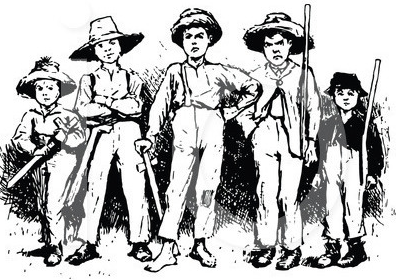
\includegraphics[width=0.3\textwidth]{img/ulica.png}
\end{wrapfigure}

Već stoljećima Pavlovom ulicom\footnote{Ako još niste, nakon natjecanja svakako
pročitajte roman \textit{Junaci Pavlove ulice}, autora Ferenca Molnara.}
vladaju dvije bande, \textit{parnokošuljaši} i \textit{neparnokošuljaši}.
Imena bandi, naravno, nisu slučajna. Parnokošuljaši su dobili to ime jer svi
dječaci u toj bandi imaju nadimke koji su parni prirodni brojevi, dok u
neparnokošuljašima svi dječaci za nadimke imaju neparne prirodne brojeve.
Svaki dječak koji živi u Pavlovoj ulici pripada jednoj od tih dviju bandi.

Mirko se danas preselio u Pavlovu ulicu i sada mora odabrati kojoj bandi će se
priključiti. On je zaključio da je bolje priključiti se onima kojih ima više.
Također, za nadimak će odabrati najmanji prirodni broj koji već nije zauzet,
tj. najmanji prirodni broj takav da u bandi kojoj će se pridružiti ne postoji
dječak s tim nadimkom. Vaš je zadatak ispisati nadimak koji je Mirko odabrao.


%%%%%%%%%%%%%%%%%%%%%%%%%%%%%%%%%%%%%%%%%%%%%%%%%%%%%%%%%%%%%%%%%%%%%%
% Input
\subsection*{Ulazni podaci}
U prvom je retku prirodan broj $N$ $(1 \le N \le 100)$, broj dječaka (ne
računajući Mirka) koji žive u Pavlovoj ulici. Možete pretpostaviti da bande
neće imati jednak broj članova.

%%%%%%%%%%%%%%%%%%%%%%%%%%%%%%%%%%%%%%%%%%%%%%%%%%%%%%%%%%%%%%%%%%%%%%
% Output
\subsection*{Izlazni podaci}
U jedinom retku ispišite Mirkov nadimak.

%%%%%%%%%%%%%%%%%%%%%%%%%%%%%%%%%%%%%%%%%%%%%%%%%%%%%%%%%%%%%%%%%%%%%%
% Scoring
\subsection*{Bodovanje}
U testnim primjerima vrijednima $10$ bodova, svi dječaci će biti parnokošuljaši.

%%%%%%%%%%%%%%%%%%%%%%%%%%%%%%%%%%%%%%%%%%%%%%%%%%%%%%%%%%%%%%%%%%%%%%
% Examples
\subsection*{Probni primjeri}
\begin{tabularx}{\textwidth}{X'X'X}
\sampleinputs{test/ulica.dummy.in.1}{test/ulica.dummy.out.1} &
\sampleinputs{test/ulica.dummy.in.2}{test/ulica.dummy.out.2} &
\sampleinputs{test/ulica.dummy.in.3}{test/ulica.dummy.out.3}
\end{tabularx}

\textbf{Pojašnjenje trećeg probnog primjera:}
Dva su parnokošuljaša i tri neparnokošuljaša, što znači da će Mirko postati
neparnokošuljaš, a njegov će nadimak biti $1$ jer je to najmanji neparan
prirodan broj i nitko nema taj nadimak.

%%%%%%%%%%%%%%%%%%%%%%%%%%%%%%%%%%%%%%%%%%%%%%%%%%%%%%%%%%%%%%%%%%%%%%
% We're done
\end{statement}

%%% Local Variables:
%%% mode: latex
%%% mode: flyspell
%%% ispell-local-dictionary: "croatian"
%%% TeX-master: "../hio.tex"
%%% End:
